\chapter{Cryptocurrency Mining}
%
\section{Overview}
%
\section{\label{sec:Bitcoin}Bitcoin}
Bitcoin~\cite{Nakamoto_bitcoin:a} is a decentralized digital currency that enables instant payments to anyone, anywhere in the world. Bitcoin uses peer-to-peer technology to operate with no central authority: transaction management and money issuance are carried out collectively by the network.

The original Bitcoin software by Satoshi Nakamoto was released under the MIT license. Most client software, derived or "from scratch", also use open source licensing.

Bitcoin is the first successful implementation of a distributed cryptocurrency, described in part in 1998 by Wei Dai on the cypherpunks mailing list. Building upon the notion that money is any object, or any sort of record, accepted as payment for goods and services and repayment of debts in a given country or socio-economic context, Bitcoin is designed around the idea of using cryptography to control the creation and transfer of money, rather than relying on central authorities.

Bitcoin is pseudonymous: the identity of each user is only their \textit{address}, which corresponds to an ECDSA public key. This address can be used to receive money from other users. Each user can spend money only if they have their corresponding private key. A set of ECDSA keypairs comprises a \textit{wallet}. A user can have multiple addresses.

Bitcoins have all the desirable properties of a money-like good. They are portable, durable, divisible, recognizable, fungible, scarce and difficult to counterfeit.

As in fiat money, transfer of value in Bitcoin happens with transactions. A transaction has inputs and outputs. An output is where the value creation happens for the receiver. An output can be later redeemed by using its designated receiver's private key and turned into an input to be used for another transaction.

\subsection{Scripts}
Bitcoin offers much more than just moving currency around. It allows us to actually move currency conditionally, where the condition can be expressed as a \emph{Bitcoin script}. Bitcoin script is a stack-based language. An example of a Bitcoin script can be seen on Figure~\ref{fig:bitcoin-script}.

\begin{figure}
  \centering
  {
    \tt
    OP\_HASH256 \\
    6fe28c0ab6f1b372c1a6a246ae63f74f931e8365e15a089c68d6190000000000 \\
    OP\_EQUAL
  }
  \caption{A Bitcoin script~\cite{gtklocker}}
  \label{fig:bitcoin-script}
\end{figure}

This script introduces two kinds of operations. The first kind is commands prefixed with \code{OP\_}. These operations are called \emph{opcodes} and they perform calculations on values on the stack. The result is pushed again to the stack. The type of the calculations are intuitive, e.g. \code{OP\_HASH256} calculates the SHA256 hash of the value on the top of the stack, \code{OP\_EQUALS} compares the top 2 values on the stack and pushes 1 if they are indeed equal or 0 otherwise. The second kind of operation is hex values. These values are simply pushed to the stack.

It is easy for the reader to see that the script of figure~\ref{fig:bitcoin-script} checks if the value on the stack is the preimage of the given hash value and returns 1 (true) or 0 (false). In practice, this output confirms the success of the evaluation. Such a script is called a \textsf{pubKeyScript}. However, in our example we assume the preimage was on the stack. The way this is implemented in Bitcoin is running another script called \textsf{scriptSig} that passes the parameters to \textsf{pubKeyScript}. Now, let's see the standard script for conventional fund transfer in Bitcoin, called \emph{pay to public key hash} (P2PKH).

% check https://en.bitcoinwiki.org/wiki/Pay-to-Pubkey_Hash for scheme and language for the following subsubsection.
%%%%% Begin from here tomorrow. After checking wiki, maybe you need to correct the paragraph above.

%%%%% v2. Now everything is kind of corrected. Please, refine the language. The whole section seems
% confusing to someone who hasn't heard about bitcoin scripts.

\subsubsection{P2PKH}
Two types of payment are referred as P2PK (pay to public key) and P2PKH (pay to public key hash).
Satoshi later decided to use P2PKH instead of P2PK for two reasons:

\begin{itemize}
  \item Elliptic Curve Cryptography is vulnerable to a modified Shor's algorithm for solving the discrete logarithm problem on elliptic curves. That means, that in the future a quantum computer might be able to retrieve a private key from a public key. By publishing the public key only when coins are spent (and assuming that addresses are not reused), such an attack is rendered ineffective.
  \item With the hash being smaller (20 bytes) it is easier to print and easier to embed into small storage mediums like QR codes.
\end{itemize}

A Bitcoin address is only a hash, so the sender can't provide a full public key in \textsf{pubKeyScript}. When redeeming coins that have been sent to a Bitcoin address, the recipient provides both the signature and the public key. The script verifies that the provided public key does hash to the hash in \textsf{pubKeyScript}, and then it also checks the signature against the public key. The reader can see the process in detail in table~\ref{tab:bitcoin}.

%%%%%%%%%%%%%%%%%%%%%%%%%%%%%%%%%%%%%%%%%%%%%%%%%%%%%%%%%%%%%%%%%%%%%%%%%%%%%%%%%%%%%%%%%%%%%
%% Don't freak out. The next lines were made with this tool: https://www.tablesgenerator.com/
%% If any debugging is needed, I strongly suggest the online tool.
%% Enjoy!
%%%%%%%%%%%%%%%%%%%%%%%%%%%%%%%%%%%%%%%%%%%%%%%%%%%%%%%%%%%%%%%%%%%%%%%%%%%%%%%%%%%%%%%%%%%%%

\begin{table}[]
  \centering
\begin{tabular}{@{}lll@{}}
\toprule
\rowcolor[HTML]{C0C0C0}
\multicolumn{1}{c}{\cellcolor[HTML]{C0C0C0}\textbf{Stack}}                                                                                                                                          & \multicolumn{1}{c}{\cellcolor[HTML]{C0C0C0}\textbf{Script}}                                                                                                                                                          & \multicolumn{1}{c}{\cellcolor[HTML]{C0C0C0}\textbf{Description}}                                                   \\ \midrule
\multicolumn{1}{|l|}{Empty}                                                                                                                                                                         & \multicolumn{1}{l|}{\begin{tabular}[c]{@{}l@{}}\textless{}sig\textgreater{}\textless{}pubKey\textgreater \\ OP\_DUP OP\_HASH160\\ \textless{}pubKeyHash\textgreater \\ OP\_EQUALVERIFY \\ OP\_CHECKSIG\end{tabular}} & \multicolumn{1}{l|}{\begin{tabular}[c]{@{}l@{}}scriptSig and\\ scriptPubKey\end{tabular}}                          \\ \midrule
\multicolumn{1}{|l|}{\begin{tabular}[c]{@{}l@{}}\textless{}pubKey\textgreater\\ \textless{}sig\textgreater{}\end{tabular}}                                                                          & \multicolumn{1}{l|}{\begin{tabular}[c]{@{}l@{}}OP\_DUP OP\_HASH160\\ \textless{}pubKeyHash\textgreater \\ OP\_EQUALVERIFY \\ OP\_CHECKSIG\end{tabular}}                                                              & \multicolumn{1}{l|}{\cellcolor[HTML]{FFFFFF}\begin{tabular}[c]{@{}l@{}}Constants\\ added\\ to stack.\end{tabular}} \\ \midrule
\multicolumn{1}{|l|}{\begin{tabular}[c]{@{}l@{}}\textless{}pubKey\textgreater\\ \textless{}pubKey\textgreater\\ \textless{}sig\textgreater{}\end{tabular}}                                          & \multicolumn{1}{l|}{\begin{tabular}[c]{@{}l@{}}OP\_HASH160\\ \textless{}pubKeyHash\textgreater \\ OP\_EQUALVERIFY \\ OP\_CHECKSIG\end{tabular}}                                                                      & \multicolumn{1}{l|}{\begin{tabular}[c]{@{}l@{}}Top stack\\ item\\ duplicated.\end{tabular}}                        \\ \midrule
\multicolumn{1}{|l|}{\begin{tabular}[c]{@{}l@{}}\textless{}pubKeyHashA\textgreater\\ \textless{}pubKey\textgreater\\ \textless{}sig\textgreater{}\end{tabular}}                                     & \multicolumn{1}{l|}{\begin{tabular}[c]{@{}l@{}}\textless{}pubKeyHash\textgreater \\ OP\_EQUALVERIFY \\ OP\_CHECKSIG\end{tabular}}                                                                                    & \multicolumn{1}{l|}{\begin{tabular}[c]{@{}l@{}}Top stack\\ item\\ hashed.\end{tabular}}                            \\ \midrule
\multicolumn{1}{|l|}{\begin{tabular}[c]{@{}l@{}}\textless{}pubKeyHash\textgreater\\ \textless{}pubKeyHashA\textgreater\\ \textless{}pubKey\textgreater\\ \textless{}sig\textgreater{}\end{tabular}} & \multicolumn{1}{l|}{\begin{tabular}[c]{@{}l@{}}OP\_EQUALVERIFY \\ OP\_CHECKSIG\end{tabular}}                                                                                                                         & \multicolumn{1}{l|}{\begin{tabular}[c]{@{}l@{}}Constant\\ added.\end{tabular}}                                     \\ \midrule
\multicolumn{1}{|l|}{\begin{tabular}[c]{@{}l@{}}\textless{}pubKey\textgreater\\ \textless{}sig\textgreater{}\end{tabular}}                                                                          & \multicolumn{1}{l|}{OP\_CHECKSIG}                                                                                                                                                                                    & \multicolumn{1}{l|}{\begin{tabular}[c]{@{}l@{}}Equality check\\ between the\\ top two stack\\ items.\end{tabular}} \\ \midrule
True                                                                                                                                                                                                & Empty.                                                                                                                                                                                                               & \begin{tabular}[c]{@{}l@{}}Signature is\\ checked for top\\ two stack items.\end{tabular}                          \\ \bottomrule
\end{tabular}
\bigskip
\caption{Bitcoin script process~\cite{p2pkh}}
\label{tab:bitcoin}
\end{table}


%%%%%%%%%%%%%%%%%%%%%%%%%%%%%%%%%%%%%%%%%%%%%%%%%%%%%%%%%%%%%%%%%%%%%%%%%%%%%%%%%%%%
%% Table finished. Let's get back to normal mode... :P!!!
%%%%%%%%%%%%%%%%%%%%%%%%%%%%%%%%%%%%%%%%%%%%%%%%%%%%%%%%%%%%%%%%%%%%%%%%%%%%%%%%%%%%
%%%%%%%%%%%%%%%%%%%%%%%%%%%%%%%%%%%%%%%%%%%%%%%%%%%%%%%%%%%%%%%%%%%%%%%%%%%%%%%%%%%%

This is the standard script for conventional fund transfer in Bitcoin. Let's say we want to make sure only Bob can satisfy this script. The \textsf{pubKeyScript} is the following: \code{OP\_DUP OP\_HASH160 <Bob's address> OP\_EQUALVERIFY OP\_CHECKSIG}. The \textsf{scriptSig} is then typically \code{<Bob's signature> <Bob's public key>}.

Bob's signature will be on the hash of the transaction (which we'll explore shortly) containing the output. The script will then duplicate his public key, check that it matches the one on the \text{pubKeyScript} and if it does, it will check that he has provided a valid signature with that public key. If all these checks pass, the stack will end up with 1 on top and the execution will be valid.

\subsection{Outputs}
An \emph{output} is a tuple ({\sf value, pubKeyScript}). The \textsf{value} refers to an amount of Bitcoin in Satoshi (where $\sf 10^8 \, Satoshi = 1 \, Bitcoin$) and \textsf{pubKeyScript} is a script which needs to be run against some stack and return 1 in order for \textsf{value} to be transferable.

\subsection{Inputs}
An input is the way an output is redeemed. Specifically, it contains 3 things:
\begin{itemize}
  \item The hash of the transaction where the output of interest is contained.
  \item An index clarifying which output in the transaction this input is referring to.
  \item A signature (called \textsf{scriptSig}) used for the validation of the output script.
\end{itemize}

For the transaction to be valid, the script inside the specified output when run on a stack with the contents of \textsf{scriptSig} should return 1. As a convention, when we talk about the value of an input we mean the value of the output it redeems.
%
%%%%%%%%%%%%%%%%%%%%%%%%%%%%%%%%%%%%%%%%%%%%%%%%%%%%%%%%%%%%%%%%%%%%%%%%%%%%%%%%%
%% Maybe the next step is Bitcoin transactions. Revise the above and start building
%% the road to mining. A! And update the READΜΕ.md! Maybe if you are bored sometime
%% fix the first pages also... It should take less than 15'...
%% Goodbye today's self, see you tomorrow.. This boring !@#$#@!$ will end sometime...
%%%%%%%%%%%%%%%%%%%%%%%%%%%%%%%%%%%%%%%%%%%%%%%%%%%%%%%%%%%%%%%%%%%%%%%%%%%%%%%%%

\subsection{Transactions}
A \emph{transaction} is a collection of inputs and outputs. It uses the sum of the inputs values' as credit to debit each output accordingly. As it makes sense, a transaction is only valid as long as all its outputs and inputs are valid. It should also be clear that the value of the outputs should not exceed the value of the inputs, otherwise we would be creating value out of thin air with new transactions. Specifically this is expressed as $\sum_{\sf i \in inputs} {\sf i.value} \ge \sum_{\sf o \in outputs} {\sf o.value}$. This is sometimes called the \emph{Law of Conservation}.

In cases where $\sum_{\sf i \in inputs} {\sf i.value} > \sum_{\sf o \in outputs} {\sf o.value}$ we call
$$\sum_{\sf i \in inputs} {\sf i.value} - \sum_{\sf o \in outputs} {\sf o.value}$$
the \emph{transaction fee}. This is paid to the miner who successfully mines a block containing the transaction. This is one of the two ways Bitcoin uses to incentivize miners. In figure~\ref{fig:transaction-internally} the reader can see the notion described above in practice.

\begin{figure}[ht]
  \centering
  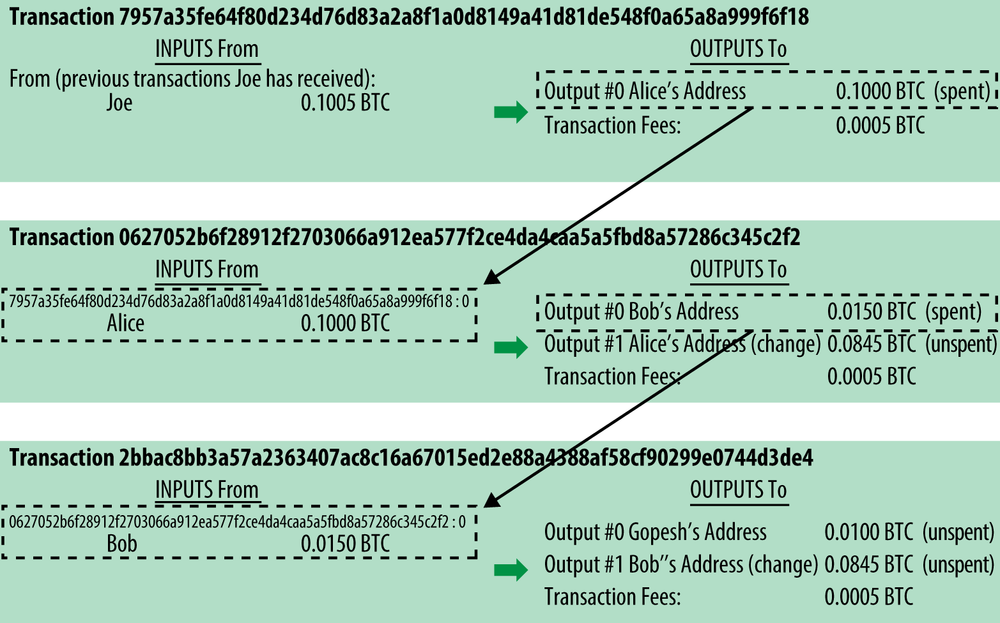
\includegraphics[width=0.9\columnwidth,keepaspectratio]{Images/transaction-internally.png}
  \caption{Transactions with their inputs and outputs.  Source:~\cite{mastering}}
  \label{fig:transaction-internally}
\end{figure}

\subsection{Blocks}
A block contains a list of transactions, the first of which is called the \emph{coinbase transaction} which is where value creation happens in Bitcoin. The miner crafts this transaction granting them some amount of Bitcoins and this transaction is going to be valid only if the block turns out valid. The amount of the \emph{coinbase transaction} is fixed by the Bitcoin protocol. However, this doesn't mean that anyone can generate Bitcoin out of thin air: we'll see shortly how it actually comes at a cost with Proof-of-Work.

\begin{figure}
  \centering
  \includegraphics[width=0.9\columnwidth,keepaspectratio]{Images/block-structure.pdf}
  \caption{The block structure.  Source:~\cite{Nakamoto_bitcoin:a}}
  \label{fig:block-structure}
\end{figure}

A block header contains mainly the hash of the previous block, a \hyperref[sec:merkle-trees]{Merkle root hash} (\hyperref[sec:merkle-trees]{section}~\ref{sec:merkle-trees}) to commit to a set of transactions, and a nonce. Blocks are always referenced by the hash of their block header.

\begin{figure}
  \centering
  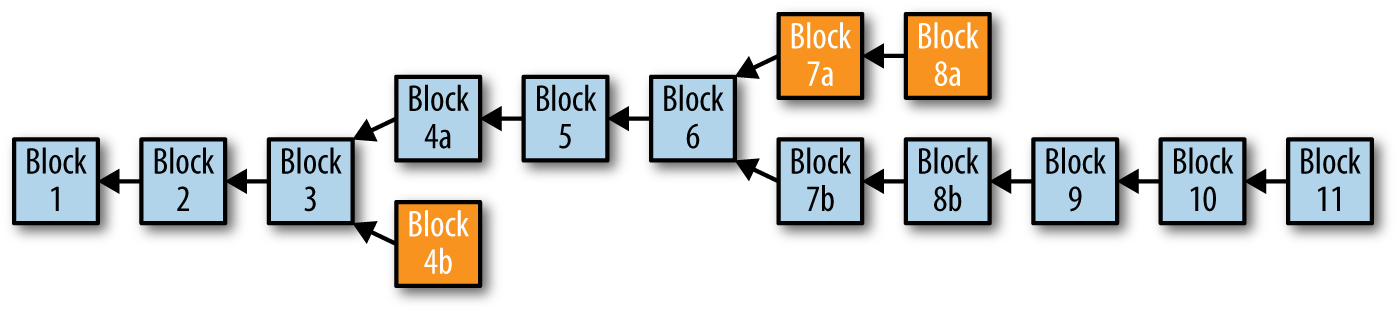
\includegraphics[width=0.9\columnwidth,keepaspectratio]{Images/blocks.png}
  \caption{A block chain. The orange blocks are orphans.  Source:~\cite{mastering}}
  \label{fig:blocks}
\end{figure}

Once a transaction has been included in a valid block it's called \emph{confirmed}.

\subsection{Blockchain}
Now, the reader can visualize the famous term \emph{blockchain}. The blockchain is a chain of blocks. The blockchain is public and it holds the history of all transactions in a cryptocurrency's network. It holds the timeline of a cryptocurrency's life. It is easy to see that, by the definition of the blockchain, there can be no parallel chains.

It's possible that there are contending chains of blocks. We then say there is a \emph{fork} on the chain. On Figure~\ref{fig:blocks}, the chain has forked on blocks 3 and 6. We call any valid blocks which are not part of our active chain \emph{orphans}. For example, on Figure~\ref{fig:blocks}, blocks 4b, 7a and 8a are orphans.

\subsection{Proof-of-Work}
The key to making Bitcoin decentralized is a technique called Proof-of-Work. Proof-of-Work was first invented in 1992 by Dwork et al.~\cite{dwork} as a measure of limiting email spam and denial-of-service attacks and later explored by Back~\cite{hashcash} as Hashcash.

We'll examine a simplified model of Hashcash in order to explore the idea. Suppose we want to send an email to someone. In order to prove we've done work, we include a header (like \code{X-Hashcash}), which (very simplistically) includes the receiver's email address, and a nonce\footnote{Hashcash headers actually contain 7 different fields which have been omitted here for simplicity. The simplified version explained here is not making the same security guarantees as Hashcash.}.
The nonce is picked so that the hash of the header $H(email || nonce)$ has its 20 most significant bits be all 0. The only feasible way to find this is by brute-forcing the nonce. Once the sender has found the nonce it's included in the header and sent.

The receiver can then very easily check whether the header hashes to a valid value. If that's so, the email it contains belongs to the receiver and the header is not being reused, then the email can be considered not spam.

To reiterate, the idea is having a series of data to commit to and a hole for the nonce, which is brute-forced to satisfy a necessary predicate on the hash, specifically that its $n$ most significant bits are all zeroes. This is exactly how Bitcoin implements Proof-of-Work. Instead of the hole being on an email header the hole is on the block header. For a block to be valid, its header has to satisfy a predicate like the above.

Bitcoin introduces a couple of differences. $n$ varies according to the block generation rate. Specifically, to translate the previous predicate to Bitcoin terminology, the hash of each block header has to satisfy $H({\sf blockHeader}) \le T$ where $T$ is called the \emph{target}. As the target goes up, the probability of being below it goes up and generating a valid block is easier. Conversely, if the target goes down it's harder to generate a valid block. To express this, in Bitcoin $\frac{1}{T}$ is called the \emph{difficulty}.

To account for the block generation rate, which Bitcoin tries to keep to 1 block per 10 minutes, every 2016 blocks the target (and subsequently the difficulty) is adjusted accordingly. The target is calculated inside the Bitcoin software and is only as a function of the blocks previously seen (frequently called their \emph{view}), so as long as the Bitcoin nodes agree on the view they'll agree on the target and all consider the same set of incoming blocks as valid.

\subsection{Simplified Payment Verification}
The size of the blockchain has reached 185GB by September 2018, which makes it a very time consuming or even infeasible process to synchronise a full node. Fortunately, a solution was proposed in the original whitepaper ~\cite{bitcoin}, which allows the creation of so-called \textit{lite nodes}.  Lite nodes only know the headers of the entire blockchain, which are constant-size for each block (80 bytes). At the time of writing of this paper, the size of all block headers was $\sim$42MB. The lite node then asks the network for transactions concerning it (e.g.\ transactions concerning a specific public key). Full nodes of the network find such transactions and return them to the requester. For each transaction, the block header of the block it's included in is returned, along with a Merkle tree proof of inclusion which the lite node can then verify. This protocol is reliable as long as an adversary does not control the network of a lite node.


%%%%%%%%%%%%%%%%%%%%%%%%%%%%%%%%%%%%%%%%%%%%%%%%%%%%%%%%%%%%%%%%%%%%%%%%%%%%%%%%
%%%%%%%%%%%%%%%%%%%%%%%%%%%%%%%%%%%%%%%%%%%%%%%%%%%%%%%%%%%%%%%%%%%%%%%%%%%%%%%%
%%%%%%%%%%%%%%%%%%%%%%%%%%%%%%%%%%%%%%%%%%%%%%%%%%%%%%%%%%%%%%%%%%%%%%%%%%%%%%%%
\section{Mining}
Bitcoin mining\footnote{It is misleading to think that there is an analogy between gold mining and bitcoin mining. The fact is that gold miners are rewarded for producing gold, while bitcoin miners are not rewarded for producing bitcoins; they are rewarded for their record-keeping services.} is the processing of transactions in the digital currency system, in which the records of current Bitcoin transactions, \textit{blocks}, are added to the record of past transactions, the \textit{blockchain}. Miners keep the blockchain consistent, complete, and unalterable by repeatedly grouping newly broadcast transactions into a block, which is then broadcast to the network and verified by recipient nodes~\cite{economist}. Each block contains a SHA-256 cryptographic hash of the previous block~\cite{economist}, thus linking it to the previous block and giving the blockchain its name.

To be accepted by the rest of the network, a new block must contain a proof-of-work ($PoW$).
The $PoW$ requires miners to find a number called a nonce, such that when the block content is hashed along with the nonce, the result is numerically smaller than the network's difficulty target~\cite{Nakamoto_bitcoin:a}. This proof is easy for any node in the network to verify, but extremely time-consuming to generate, as for a secure cryptographic hash, miners must try many different nonce values before meeting the difficulty target.

The primary purpose of mining is to set the history of transactions in a way that is computationally impractical to modify by any one entity. By downloading and verifying the blockchain, bitcoin nodes are able to reach consensus about the ordering of events in bitcoin~\cite{wiki}.

Every 2,016 blocks (approximately 14 days at roughly 10 min per block), the difficulty target is adjusted based on the network's recent performance, with the aim of keeping the average time between new blocks at ten minutes. In this way the system automatically adapts to the total amount of mining power on the network. Between 1 March 2014 and 1 March 2015, the average number of nonces miners had to try before creating a new block increased from 16.4 quintillion to 200.5 quintillion~\cite{difficulty_history}.

The proof-of-work system, alongside the chaining of blocks, makes modifications of the blockchain extremely hard, as an attacker must modify all subsequent blocks in order for the modifications of one block to be accepted. As new blocks are mined all the time, the difficulty of modifying a block increases as time passes and the number of subsequent blocks (also called confirmations of the given block) increases~\cite{economist}.

Mining is also the mechanism used to introduce Bitcoins into the system: Miners are paid any transaction fees as well as a "subsidy" of newly created cryptocoins. This both serves the purpose of disseminating new cryptocoins in a decentralized manner as well as motivating people to provide security for the system~\cite{wiki}.

Originally, Bitcoin mining was conducted on the \textit{CPUs} of individual computers, with more cores and greater speed resulting in more profitability. After that, the system became dominated by multi-graphics card systems, then field-programmable gate arrays (\textit{FPGAs}) and finally application-specific integrated circuits (\textit{ASICs}), in the attempt to find more hashes per hour with less electrical power usage.

Due to this constant escalation, it has become hard for prospective new miners to start. This adjustable difficulty is an intentional mechanism created to prevent inflation. To get around that problem, individuals often work in mining pools.

Bitcoin generally started with individuals and small organizations mining. At that time, start-up could be enabled by a single high-end gaming system. Now, however, larger mining organizations might spend tens of thousands on one high-performance, specialized application-specific integrated circuit.

That creates a problem. In a system, which from its creation, it is supposed to distribute power among users, there has been a great power concentration in the hands of big companies, like Bitfury or 21, that develop ASICs to mine bitcoin. Because of the extreme cost of ASICs and extreme hashrate, someone who uses a multi-graphics card system or a $CPU$ is out of competition. As a result of this, independent miners have largely dried up.

%
\section{Egalitarian Mining}
Let's consider several contexts where an adversary has an upper hand over the defender by using special hardware in an attack. These include password processing, hard-drive protection, cryptocurrency mining, resourse sharing, code obfuscation, etc. Memory-hard computing is a generic paradigm, which can protect the defender against attacks in the aforementioned contexts. Every task is amalgamated with a certain procedure requiring intensive access to $RAM$ both in terms of size and bandwidth, so that transferring the computation to $GPU$, $FPGA$, and even $ASIC$ brings little or no cost reduction. Cryptographic schemes that run in this framework become \emph{egalitarian} in the sense that both users and attackers are equal in the price-performance ratio conditions. When the cryptographic scheme is a hash fuction used for cryptocurrency mining, then we refer to this notion as \emph{egalitarian mining}.

But let's step back a little and think about the need for such a notion. Do we actually need it? Is egalitarian mining a way to destroy competition? Is it unfair? Shouldn't a miner be rewarded for the extra money he invested?

Many questions like the above have been asked and usually the answer is not descriptive enough of what really memory-hardness introduces to the world. We will try here to demonstrate exactly what it means for a cryptocurrency to offer egalitarian mining.

\emph{Egalitarian mining does not destroy competition.} The miner who invests more in hardware, is rewarded more. Each individual miner is rewarded according to the computation power he offers to the community. The real difference is that it is really easy for people to start mining with a single high-end gaming system. Hobbyists, who want to support the community are welcome to mine. In bitcoin system, this option is not available. In order to support the community by mining, you have to invest a lot of money on ASICs to be competitive. That means, that in general, the mining to support the Bitcoin project or for fun, is dead.

This is hurtful for a system, which by design is supposed to bring decentralization in the financial market. That is, because without hobbyists we are actually left with big companies handling almost all of the mining. Companies will comply with regulations that the government of each country enforces and cannot be expected to react and inspire political movements. Since countries can and they have, historically, collaborated against threats, a union of countries who can enforce regulations to companies that control more than 51\% of the hashing power, can bring a cryptocurrency to its knees if seen as a threat. That scenario, does not fit in most definitions of security.

One of the reasons that cryptocurrencies have a bootstrapping period is because they need a big support society to distribute mining in order to guarantee security. When the total hashing power is a few high-end gaming systems, aquaring 51\% of the hashing power is feasible. As the support expands, the security is satisfied for all practical purposes. But when mining is dominated by companies then a totally trustless system gaves birth to a trusted party. That's against the motivation for the inception of a cryptocurrency and it raises questions like "\emph{Why should I trust the mining companies and support this cryptocoin? Do I trust my bank more? After all, my bank is just another company...}"

We are focusing on mining, but one should think about the possibilities of a proof-of-work mechanism in order to understand the contribution of a memory-hard hash function. The proof of work mechanism is actually a voting system. Users vote for the right order of the transactions, for enabling new features in the protocol and for the honest money supply distribution. Therefore, it is important that during the voting process all participant have equal voting rights.

To sum up, for reasons of security and decentralization, it is healthy for some cryptocurrency's mining power to be distributed among users. Memory-hardness sustains the competition, but it makes it less harsh and keeps the door open for hobbyists to support the community. It is extremely difficult for the corporate mining to aquire tremendous power for two reasons, and that is essential in a trustless system that aims to stay trustless. The reasons are: a) it is not that lucrative for companies. If someone makes a big investment, he will get big rewards, but not insanely huge rewards leaving every hobbyist out of the mining society. b) Even if a lot of companies decide to participate, it is extremely difficult for them to aquire a combined 51\% of the total hashing power without destroying the "support mining" or "fun mining".

Memory-hardness defends a system against the aforementioned prospect and thus strengthens the notion of any proof-of-work cryptocurrency's security. Furthermore, no matter how much someone trusts the corporations involved, security is a binary state. A system cannot be secure against malicious attackers and insecure against other "noble" parties. It is either secure or insecure. And if the prospect of an attack exists, then security collapses.
%
\section{Monero}
Monero (\emph{XMR}) is a decentralised open-source cryptocurrency forked from Bytecoin in April 2014. The project's fundamental feature is privacy - it aims to be a digital medium of exchange with untraceable payments, unlinkable transactions and resistance to blockchain analysis. The persons behind a Monero transaction are not known; this results in considerable increase of privacy compared to Bitcoin and its forks~\cite{monerodef}.

Monero is actively encouraged to those seeking financial privacy, since payments and account balances remain entirely hidden, which is not the standard for most cryptocurrencies.\\

\noindent Monero is~\cite{monero}:
\begin{description}
  \item [Untraceable] Monero uses a digital signature scheme called "ring signatures", which shuffles users' public keys in order to eliminate the possibility to identify a particular user.
  \item [Unlinkable] Monero employs a specific protocol which generates multiple unique one-time addresses that can only be linked by the payment receiver and are unfeasable to be revealed through blockhain analysis.
  \item [Secure] Monero is cryptographically secured. Moreover, the design of the algorithm used, consists in tremendous computational and electric capibilities that an adversary would need to even try to steal funds.
  \item [Private] Privacy is basically provided by the idea of anonymous transactions without any obligations to cooperate with third parties.
  \item [Analysis Resistant] Monero's blockchain analysis resistance results from unlinkability, which is achieved by using a modified version of the Diffie-Hellman exchange protocol that generates multiple one-time public addresses that can only be simply gathered by the message receiver, but hardly analyzed by confused foreigners inside the block explorer.
\end{description}
%
In Monero a wallet is called an account and it is a private account owned and operated by a Monero user. An account contains all of the Monero transactions a user has sent and received. Some user's account balance is a sum of all the Monero received, less the Monero sent.

A Monero account has two balances, a locked and an unlocked balance. The unlocked balance contains funds that can be spent immediately, and the locked balance contains funds that can't be spent right now. A Monero user may receive a transaction that has an unlock time set, or he/she may have sent some Monero and are waiting for the change to come back to his/her wallet, both situations that could lead to those funds being locked for a time.

An account resides only under user's control, normally on his/her computer, and cannot be accessed by anyone else if he/she practices good security~\cite{getmonero}.

Monero uses a proof-of-work mechanism to issue new coins and
incentivize miners to secure the network and validate transactions.
One key part, for Monero project to offer the above, is a proof-of-work algorithm called CryptoNight, developed by the CryptoNote
project~\cite{citeulike:14139412}. On top of typical security attributes, this algorithm is also suspected to be memory-hard. The aim of this work is to study the memory-hardness property of this algorithm.
%
\section{CryptoNote}
CryptoNote, as described in the bitcoin forum~\cite{btcforum}, is the technology that allows creation of privacy-centric cryptocurrencies. The level of anonymity provided by CryptoNote isn't possible with Bitcoin code base by design. Bytecoin (\emph{BCN}) was the CryptoNote reference implementation, and \emph{XMR} is based on \emph{BCN}'s code.

Two of the main features of CryptoNote are ring signatures that mask sender identities by mixing and one-time keys that make transactions unlinkable. Their combined effect gives a high degree of anonymity without any extra effort on the part of the user.

Unlike Bitcoin, user's funds are not held in the address he/she gives out to others. Instead, every time he/she receives a payment it goes to an unlinkable address generated with random numbers. When he/she decides to spend the funds in that one-time address, the amount will be broken down and the components will be indistinguishable from identical outputs in the blockchain.

For example if $556.44$ \emph{XMR} are sent, the protocol will break it down into $500 + 50 + 6 + 0.4 + 0.04$ and a ring signature will be performed with other $500$'s, $50$'s, $6$'s, $0.4$'s, and $0.04$'s in the blockchain. Unlike the "CoinJoin" mixing method~\cite{coinjoin}, CryptoNote mixes outputs not transactions. This means no other senders need to be participating with some user at the same time or with the same amounts. Any arbitrary amount sent at any time can always be rendered fundamentally indistinguishable (a mathematical proof is given in the white paper)~\cite{citeulike:14139412}.

The degree of anonymity is also a choice rather than decided by the protocol: do you want to be hidden as one among five or one among fifty? The size of the signature grows linearly as $O(n+1)$ with the ambiguity so greater anonymity is paid for with higher fees to miners.\\

\noindent Ring signatures are explained below. We will start with a normal signature scheme shown in \hyperref[fig:normal_sig]{Fig.}~\ref{fig:normal_sig}. Reproduced from CryptoNote~\cite{cryptonote}:\\
\begin{figure}[ht]
  \centering
  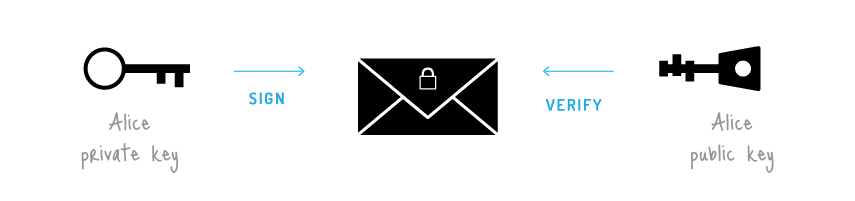
\includegraphics[width=0.9 \columnwidth,keepaspectratio]{Images/CryptoNote/normal_sig.png}
  \caption{Normal signature: One participant, which allows one-to-one mapping.}
  \label{fig:normal_sig}
\end{figure}\\
In \hyperref[fig:ring_sig]{Fig.}~\ref{fig:ring_sig} we show the ring signature concept:\\
\begin{figure}[ht]
  \centering
  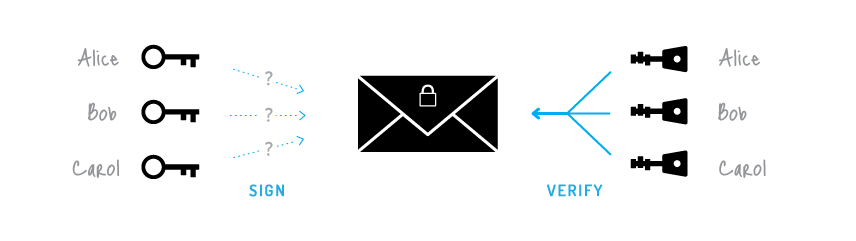
\includegraphics[width=0.9 \columnwidth,keepaspectratio]{Images/CryptoNote/ring_sig.png}
  \caption{Ring signature: Only proves that a signer belongs to a group.}
  \label{fig:ring_sig}
\end{figure}\\
The result is shown in \hyperref[fig:result]{Fig.}~\ref{fig:result}. The reader can think of it as decentralized and trustless mixing.
%% In the final document the following line needs to be uncommented in order to show the figures properly.
%\newpage
\begin{figure}[ht]
  \centering
  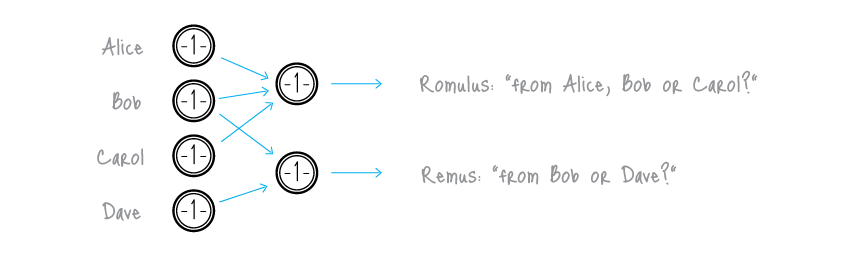
\includegraphics[width=0.9 \columnwidth,keepaspectratio]{Images/CryptoNote/result.png}
  \caption{High level of anonymity in cryptocurrency transactions.}
  \label{fig:result}
\end{figure}

%% Uncomment the following line in the final document, if it is placed after a figure. Looks bad otherwise.
%\noindent
Now that we have seen the whole concept, it is time to see what a transaction looks like in this context. Again reproduced from CryptoNote~\cite{cryptonote}, we will subjoin an example and a figure showing the details of a transaction from Bob to Carol.

Bob decides to spend an output, which was sent to the one-time public key. He needs Extra \textbf{(1)}, TxOutNumber \textbf{(2)}, and his Account private key \textbf{(3)} to recover his one-time private key \textbf{(4)}.

When sending a transaction to Carol, Bob generates its Extra value by random \textbf{(5)}. He uses Extra \textbf{(6)}, TxOutNumber \textbf{(7)} and Carol's Account public key \textbf{(8)} to get her Output public key \textbf{(9)}.

In the input Bob hides the link to his output among the foreign keys \textbf{(10)}. To prevent double-spending he also packs the Key image, derived from his One-time private key \textbf{(11)}.

Finally, Bob signs the transaction, using his One-time private key \textbf{(12)}, all the public keys \textbf{(13)} and Key Image \textbf{(14)}. He appends the resulting Ring Signature to the end of the transaction \textbf{(15)}.

The example above is illustrated in \hyperref[fig:transaction]{Fig.}~\ref{fig:transaction}.\\
\begin{figure}[ht]
  \centering
  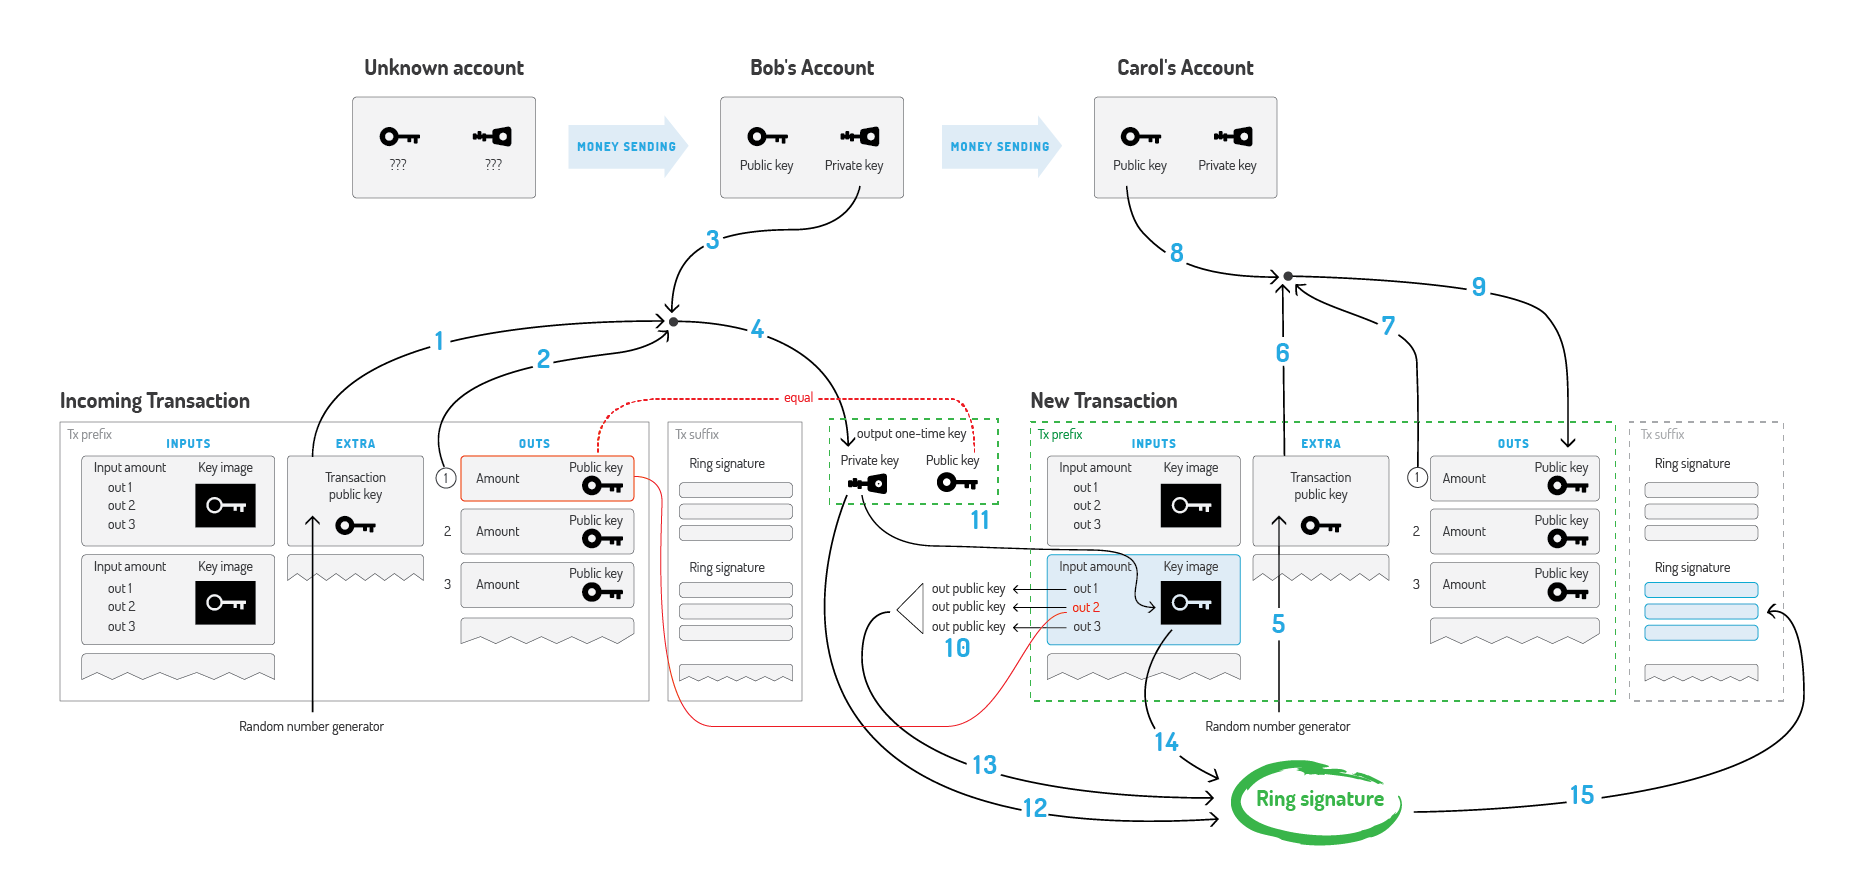
\includegraphics[width=0.9 \columnwidth,keepaspectratio]{Images/CryptoNote/transaction.png}
  \caption{A sample transaction from Bob to Carol.}
  \label{fig:transaction}
\end{figure}
%
